\documentclass[aspectratio=169, table]{beamer}

\graphicspath{{../../images/}}
%\usepackage[beamertheme=./praditatheme]{Pradita}

\usetheme{Pradita}

\subtitle{IF231303-Software Architecture}
%\date[Serial]{\scriptsize {PRU/SPMI/FR-BM-18/0222}}
\author[Pradita]{\small {\textbf{Alfa Yohannis}}}
\title{\huge Chapter-12:\\Microservices}
\author{Alfred Gerald, Lucky Rusandana, Inzaghi Posuma\\Alfa Yohannis}

\begin{document}

    \frame{\titlepage}

    \begin{frame}
        \frametitle{Microservices}
        \vspace{25pt}
        \begin{itemize}
            \item Microservices adalah sebuah arsitektur perangkat lunak yang membagi sebuah aplikasi besar menjadi beberapa komponen kecil yang independen.
            \item Komponen-komponen tersebut dapat berkomunikasi satu sama lain melalui antarmuka yang didefinisikan secara jelas.
            \item Setiap komponen atau layanan dalam arsitektur microservices memiliki tugas dan tanggung jawab tertentu yang dapat dijalankan secara mandiri.
            \item Komponen dapat diubah tanpa mempengaruhi layanan lain dalam aplikasi.
            \item Komunikasi antara layanan biasanya dilakukan melalui protokol HTTP atau pesan.
        \end{itemize}
    \end{frame}

    \section{Microservices}
    %        \framesubtitle{}
    \begin{frame}{Microservices}
        \vspace{30pt}
        \begin{columns}
            \column{0.25\textwidth}
            \url{https://microservices.io}
            \column{0.75\textwidth}
                    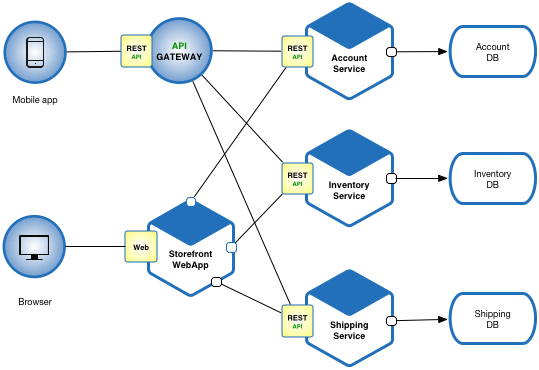
\includegraphics[width=\textwidth]{../../images/Microservice_Architecture}
        \end{columns}
    \end{frame}

    \begin{frame}
        \frametitle{Kelebihan Microservices}
        Berikut adalah beberapa kelebihan dari menggunakan arsitektur microservices dalam pengembangan perangkat lunak:
        \begin{itemize}
            \item \textbf{Scalability}: Arsitektur microservices memungkinkan skalabilitas yang lebih baik dibandingkan dengan monolithic architecture.
            \item \textbf{Fleksibilitas}: Dalam arsitektur microservices, setiap layanan dapat dikembangkan secara terpisah tanpa mempengaruhi layanan lainnya.
            \item \textbf{Toleransi Kesalahan}: Jika terjadi kesalahan pada satu layanan, maka layanan lainnya masih dapat berjalan normal dan tidak terganggu.
        \end{itemize}
    \end{frame}

    \begin{frame}
        \frametitle{Kelebihan Microservices (2)}

        \begin{itemize}
            \item \textbf{Skalabilitas tim}: Dalam arsitektur microservices, tim pengembang dapat fokus pada layanan tertentu dan membuat perubahan dengan cepat tanpa harus memikirkan bagaimana perubahan tersebut akan memengaruhi layanan lain dalam aplikasi.
            \item \textbf{Teknologi yang beragam}: Dalam arsitektur microservices, setiap layanan dapat menggunakan teknologi yang berbeda.
            \item \textbf{Skalabilitas bisnis}: Dalam arsitektur microservices, setiap layanan dapat berjalan secara independen.
        \end{itemize}
    \end{frame}

    \begin{frame}
        \frametitle{Kekurangan Microservices}
        \begin{itemize}
            \item \textbf{Kompleksitas}: Penggunaan arsitektur microservices dapat meningkatkan kompleksitas sistem secara keseluruhan.
            \item \textbf{Koordinasi yang lebih rumit}: Akibat dari sistem yang menjadi kompleks, koordinasi antar layanan mungkin agak lebih rumit.
            \item \textbf{Perlu banyak automation}: Microservices juga membutuhkan sistem automation yang cukup tinggi untuk bisa melakukan deployment.
            \item \textbf{Biaya}: Penggunaan arsitektur microservices dapat memerlukan biaya yang lebih tinggi.
        \end{itemize}
    \end{frame}



    \begin{frame}
        \frametitle{Aplikasi Microservices}
        \vspace{25pt}
        \begin{columns}
            \column{0.5\textwidth}
            \textbf{Platform E-commerce}
            \begin{itemize}
                \item \textbf{Amazon}: Pemrosesan pesanan, pembayaran, katalog produk.
                \item \textbf{eBay}: Pencarian, manajemen pengguna, transaksi.
            \end{itemize}
            \textbf{Layanan Streaming}
            \begin{itemize}
                \item \textbf{Netflix}: Akun pengguna, rekomendasi konten, streaming.
                \item \textbf{Spotify}: Rekomendasi musik, daftar putar, pembayaran.
            \end{itemize}

            \column{0.5\textwidth}
            \textbf{Media Sosial}
            \begin{itemize}
                \item \textbf{Twitter}: Pemrosesan tweet, timeline, notifikasi.
                \item \textbf{LinkedIn}: Profil pengguna, koneksi, rekomendasi pekerjaan.
            \end{itemize}
            \textbf{Telekomunikasi}
            \begin{itemize}
                \item \textbf{AT\&T}: Infrastruktur jaringan, layanan pelanggan, penagihan.
                \item \textbf{Verizon}: Manajemen jaringan, dukungan pelanggan.
            \end{itemize}
        \end{columns}
    \end{frame}

    \begin{frame}
        \frametitle{Kesimpulan}
        \vspace{25pt}
        \begin{itemize}
            \item \textbf{Microservices} adalah pendekatan arsitektur perangkat lunak yang membagi aplikasi besar menjadi komponen-komponen kecil yang independen; pada umumnya dalam bentuk \textit{web services}.
            \item \textbf{Kelebihan} dari menggunakan arsitektur microservices meliputi skalabilitas, fleksibilitas, toleransi kesalahan, skalabilitas tim, teknologi yang beragam, dan skalabilitas bisnis.
            \item Namun, terdapat juga beberapa \textbf{kekurangan} seperti kompleksitas, koordinasi yang lebih rumit, kebutuhan akan otomasi yang tinggi, dan biaya yang lebih tinggi.
            \item Meskipun demikian, banyak perusahaan terkemuka seperti Amazon, Netflix, Twitter, dan AT\&T yang telah berhasil \textbf{menerapkan} arsitektur microservices dalam produk dan layanan mereka.
        \end{itemize}
    \end{frame}

\end{document}
